\documentclass[aspectratio=169,11pt]{beamer}
\usetheme{metropolis}
\usepackage[T1]{fontenc}
\usepackage[utf8]{inputenc}
% Times-family fonts for all slides (house style)
\usefonttheme{professionalfonts}
\usepackage{newtxtext,newtxmath}
\renewcommand{\familydefault}{\rmdefault}
\usepackage{booktabs}
\usepackage{amsmath,amssymb}
\usepackage{graphicx}
\usepackage{xcolor}

\definecolor{luhblue}{RGB}{21,101,192}
\definecolor{alertred}{RGB}{198,40,40}
\setbeamercolor{frametitle}{bg=luhblue, fg=white}
\metroset{progressbar=frametitle, block=fill}
\setbeameroption{hide notes}   % default build is clean; notes extracted for narration

\graphicspath{{./figures/pce_uq/}{./figures/}{./figures/topic6_bayesian/}{./figures/topic9_kl/}{./figures/topic13_comparison/}}

\title{Reliability Assessment of the JAXA H3 Fairing under Manufacturing Variability}
\subtitle{Polynomial Chaos Expansion as a Stochastic FEM Surrogate}
\author{Keisuke Nishioka}
\institute{Stochastic Finite Element Methods --- Dr.\ Z.\ Zheng / Prof.\ U.\ Nackenhorst \quad LUH SoSe\,2026}
\date{}

\begin{document}

\maketitle
\note{Good morning. I will present my project for the Stochastic Finite Element Methods course: a reliability assessment of the JAXA H3 rocket fairing under manufacturing variability, using polynomial chaos expansion as a stochastic finite element surrogate. The question is simple to state: given that the material properties of a composite fairing vary from manufacturing, how does that variability propagate into the structural response, and is the structure reliable? I answer this with a non-intrusive polynomial chaos expansion built on top of an Abaqus model.}

\begin{frame}{Motivation: manufacturing variability in composite fairings}
\begin{columns}[T]
\begin{column}{0.6\textwidth}
\begin{itemize}
  \item The H3 fairing is a \textbf{CFRP / aluminum-honeycomb sandwich}.
  \item Material properties vary from manufacturing: fiber volume fraction, cure cycle, adhesive film thickness.
  \item This uncertainty propagates into \textbf{stress, damage, and deflection} --- and hence reliability.
\end{itemize}
\vspace{0.5em}
\textbf{Goal:} quantify how five uncertain material parameters propagate to the structural response, treating the Abaqus model as a black box.
\end{column}
\begin{column}{0.4\textwidth}
\begin{alertblock}{Stochastic FEM}
Propagate input uncertainty through a deterministic FE model to obtain response statistics and a failure probability.
\end{alertblock}
\end{column}
\end{columns}
\end{frame}
\note{Why does this matter? The H3 fairing is a carbon-fiber-reinforced-plastic skin bonded to an aluminum honeycomb core. The properties of the CFRP and of the adhesive bond are inherently variable, because of fiber-volume-fraction fluctuations, cure-cycle variations, and adhesive film-thickness inconsistencies. These uncertainties propagate into the stress, the damage, and the deflection, and therefore into the reliability of the structure. My goal is to quantify how five uncertain material parameters propagate to the structural response, treating the existing high-fidelity Abaqus model purely as a black box.}

\begin{frame}{The structure: H3 payload fairing --- design \& FE model}
\begin{columns}[T]
\begin{column}{0.36\textwidth}
\begin{center}
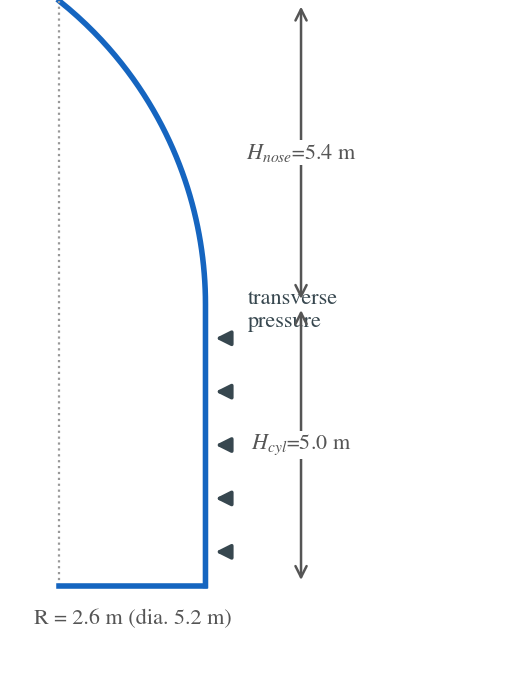
\includegraphics[height=0.74\textheight]{fairing_geometry.png}
\end{center}
\end{column}
\begin{column}{0.62\textwidth}
\scriptsize
\textbf{Geometry} \quad (CFRP / Al-honeycomb sandwich)
\begin{itemize}\itemsep0pt
  \item Diameter 5.2~m; ogive nose $H_\text{nose}=5.4$~m, cylinder $H_\text{cyl}=5.0$~m
  \item CFRP face sheets 0.6--1.4~mm; Al-honeycomb core 8~mm
\end{itemize}
\vspace{0.2em}
\textbf{Material constants}
\begin{itemize}\itemsep0pt
  \item CFRP skin (orthotropic LAMINA): $E_1\!\approx\!146$~GPa, $E_2\!\approx\!10$~GPa,
        $G_{12}\!\approx\!5.2$~GPa, $\nu_{12}=0.3$
  \item Al-honeycomb core: orthotropic --- stiff out-of-plane ($E_3$), soft in-plane
  \item Adhesive --- cohesive zone (BK, $\eta=2.284$): $K_n=10^{6}$~N/mm$^3$,
        $G_{Ic}=0.3$~N/mm, $t_n=50$~MPa
\end{itemize}
\vspace{0.2em}
\textbf{Boundary conditions \& load}
\begin{itemize}\itemsep0pt
  \item Base ring \textbf{clamped}; skins--core tied via the cohesive interface
  \item Step 1: transverse \textbf{pressure}; \; Step 2: incremental load
\end{itemize}
\vspace{0.2em}
Five constants ($E_1,G_{12},K_n,G_{Ic},t_n$) are treated as \textbf{uncertain} (next slides).
\end{column}
\end{columns}
\end{frame}
\note{Concretely, this is the structure. On the left, the H3 launch vehicle, with the payload fairing at the nose highlighted. On the right, a representative wall panel of that fairing: a carbon-fiber skin, an aluminum-honeycomb core, and a second carbon-fiber skin, all bonded with a structural adhesive modeled as a cohesive zone. Manufacturing variability lives in the skin stiffness and in the adhesive bond, and that is exactly what we propagate.}

\begin{frame}{Objectives}
\textbf{Forward UQ (core):}
\begin{enumerate}
  \item Construct PCE surrogates (deg.~2 \& 3) via \textbf{Smolyak sparse quadrature}; validate convergence.
  \item Identify the dominant parameter via \textbf{Sobol global sensitivity analysis}.
  \item Assess structural reliability --- $P_f$ and $\beta$.
\end{enumerate}
\vspace{0.4em}
\textbf{Extensions:}
\begin{enumerate}\setcounter{enumi}{3}
  \item[\textbf{T6}] \textbf{Bayesian inverse}: infer $E_1$ from stress measurements using PCE as likelihood.
  \item[\textbf{T9}] \textbf{KL random field}: represent $E_1(x,y)$ spatially; assess conservative-ness of scalar model.
  \item[\textbf{T13}] \textbf{Surrogate comparison}: PCE vs.\ GP vs.\ NN over training sizes $N=10$--$286$.
\end{enumerate}
\end{frame}
\note{The study has three core objectives and three extensions, all built around the same H3 fairing model. The core objectives are: construct polynomial-chaos surrogates at degree two and three via Smolyak sparse quadrature and validate convergence; identify the dominant parameter via Sobol sensitivity analysis; and assess reliability. The three extensions use the same forward model as a building block. Topic 6 uses the PCE as a likelihood evaluator in a Bayesian inverse problem to infer E1 from stress measurements. Topic 9 replaces the scalar E1 assumption with a spatially correlated random field via Karhunen-Loeve expansion and checks whether the scalar analysis is conservative. Topic 13 systematically compares PCE, Gaussian Process, and Neural Network surrogates as a function of training data size.}

\begin{frame}{Approach at a glance}
\begin{center}
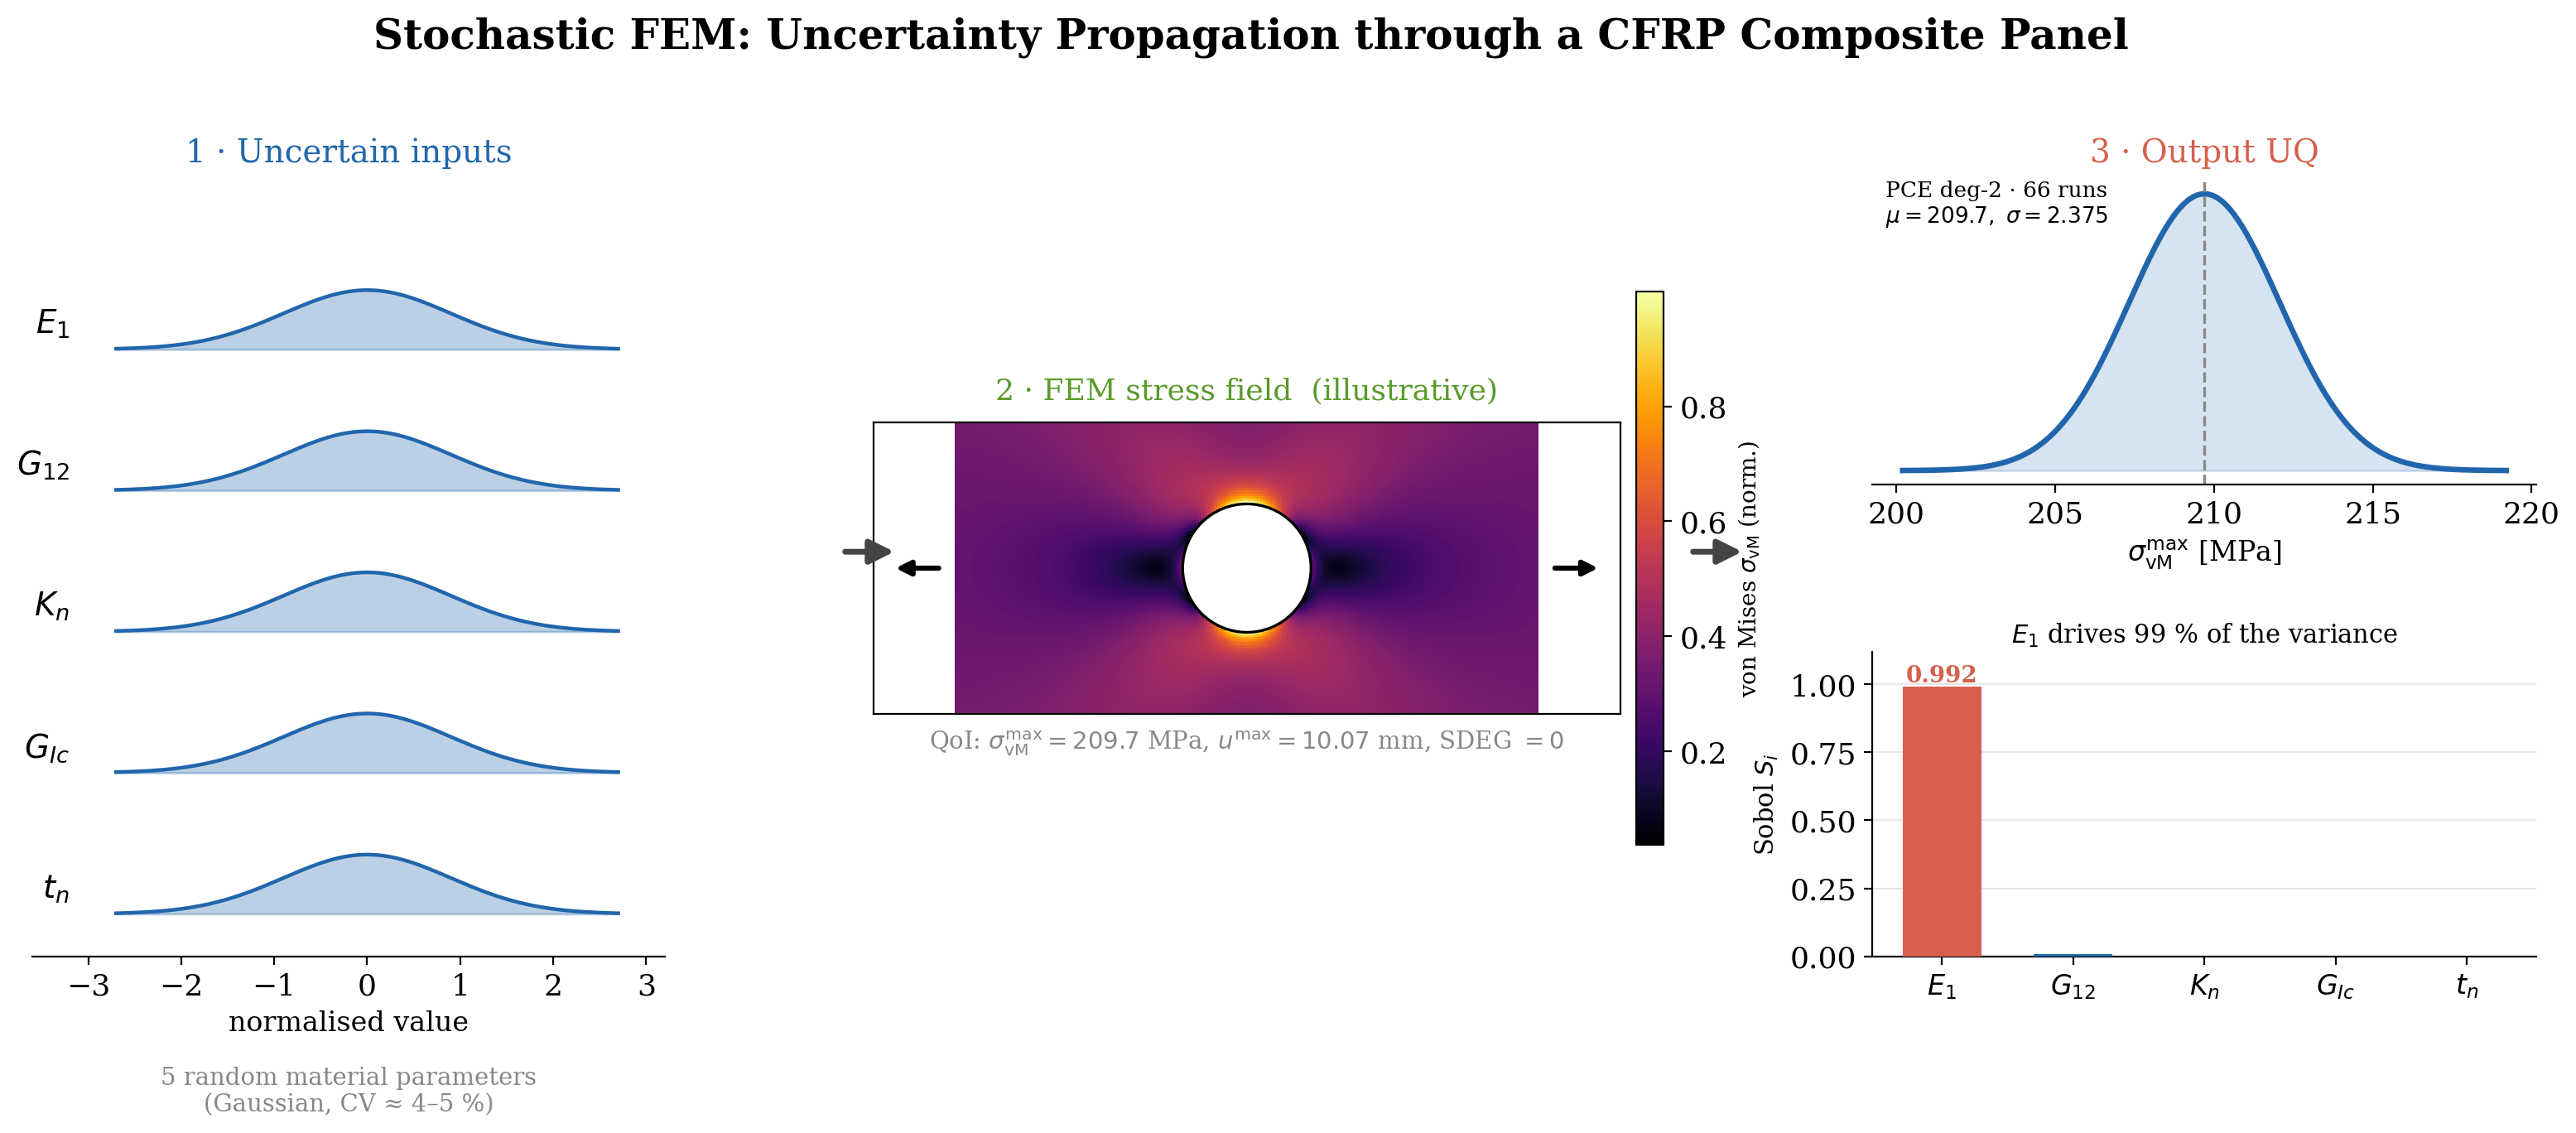
\includegraphics[width=\linewidth]{hero_sfem_pipeline.png}
\end{center}
\vspace{-0.4em}
{\footnotesize Non-intrusive pipeline: sample the five uncertain material parameters, propagate each draw through the deterministic Abaqus model, and recover the response distribution and Sobol indices. The stress field is illustrative; $E_1$ governs over 99\% of the variance.}
\end{frame}
\note{Here is the whole approach on one slide. On the left, the five uncertain material parameters, each given as a Gaussian distribution. In the middle, the deterministic finite-element model, which we treat as a black box and evaluate at quadrature nodes; the stress field shown is illustrative. On the right, the two things we recover: the probability distribution of the maximum von Mises stress, and the Sobol sensitivity indices, which reveal that the first stiffness E1 governs more than ninety-nine percent of the output variance. Everything that follows is detail on these three stages.}

\begin{frame}{Method: Polynomial Chaos Expansion}
For a response $Y=\mathcal{M}(\xi)$ with random inputs $\xi\in\mathbb{R}^d$:
\[
  Y \approx \hat Y = \sum_{\alpha\in\mathcal A} c_\alpha \Psi_\alpha(\xi),
  \qquad P=\binom{d+p}{p}.
\]
\begin{itemize}
  \item $\Psi_\alpha$: \textbf{Hermite} polynomials --- orthogonal w.r.t.\ the Gaussian measure.
  \item Orthogonality $\Rightarrow$ mean $=c_0$, variance $=\sum_{\alpha\neq0}c_\alpha^2\,\mathbb{E}[\Psi_\alpha^2]$.
  \item \textbf{Sobol indices follow analytically} from grouped squared coefficients --- no extra model runs.
\end{itemize}
\end{frame}
\note{Here is the method. For a model response Y depending on a random input vector xi, polynomial chaos approximates Y as a finite sum of coefficients times orthogonal polynomial basis functions. For Gaussian inputs, those basis functions are Hermite polynomials. The crucial point is not the polynomial form but the orthogonality: because the basis is orthogonal with respect to the Gaussian measure, the coefficients are the spectral projections of the response. So the mean is read directly from the zeroth coefficient, and the variance from the sum of the remaining squared coefficients. The Sobol sensitivity indices then follow analytically, as partial sums of those squared coefficients grouped by the variables each term activates --- with no additional model evaluations. That is the decisive advantage of polynomial chaos over a generic regression surrogate.}

\begin{frame}{Method: Smolyak sparse quadrature}
\begin{columns}[T]
\begin{column}{0.52\textwidth}
Full tensor-product Gauss--Hermite quadrature needs $n_q^d$ points --- prohibitive in $d=5$.
Smolyak sparse grids keep polynomial exactness while slashing the count.
\vspace{0.5em}

{\footnotesize Negative sparse weights handled by least-squares regression fallback.}
\end{column}
\begin{column}{0.48\textwidth}
\begin{table}
\centering\small
\begin{tabular}{lccc}
\toprule
$p$ & Full & Sparse & Reduction \\
\midrule
2 & $3^5{=}243$  & \textbf{66}  & $3.7\times$ \\
3 & $4^5{=}1024$ & \textbf{286} & $3.6\times$ \\
\bottomrule
\end{tabular}
\end{table}
\end{column}
\end{columns}
\end{frame}
\note{To build the surrogate we need to sample the model at quadrature nodes. A full tensor-product Gauss-Hermite rule would need n-q to the power d points --- for five parameters at degree three that is four to the fifth, over a thousand Abaqus runs, which is prohibitive. The Smolyak sparse grid keeps the same polynomial exactness but cuts the number of evaluations dramatically: from two hundred forty-three down to sixty-six at degree two, and from over a thousand down to two hundred eighty-six at degree three, roughly a factor of three point seven. Where the sparse rule produced negative quadrature weights, I fell back to least-squares regression to fit the coefficients.}

\begin{frame}{Five uncertain input parameters}
\begin{table}\centering\small
\begin{tabular}{llccc}
\toprule
Parameter & Description & Nominal & CoV & \\
\midrule
$E_1$    & fiber-direction modulus     & 146{,}000 MPa & \textbf{5\%}  & \\
$G_{12}$ & in-plane shear modulus      & 5{,}200 MPa   & 10\% & \\
$K_n$    & cohesive normal stiffness   & $10^6$ N/mm$^3$ & 15\% & \\
$G_{Ic}$ & Mode-I fracture energy      & 0.3 N/mm      & 20\% & \\
$t_n$    & cohesive strength           & 50 MPa        & 15\% & \\
\bottomrule
\end{tabular}
\end{table}
\vspace{0.3em}
Independent \textbf{truncated-normal} variables, bounded at $[0.5\mu,\,1.5\mu]$ --- stiffnesses are strictly positive, and flight hardware is screened against inspection limits.
\end{frame}
\note{The five uncertain parameters are these. The fiber-direction modulus E1, the in-plane shear modulus G12, the cohesive-zone normal stiffness Kn, the Mode-I fracture energy GIc, and the cohesive strength tn. They are modeled as independent truncated-normal variables, bounded between fifty and one hundred fifty percent of nominal. The truncation is deliberate: stiffnesses and fracture energies are strictly positive, so an unbounded Gaussian would assign probability to non-physical negative draws; and material accepted for flight hardware is screened against incoming-inspection limits, so extreme outliers are not representative. The assumed coefficients of variation follow the usual ordering for CFRP --- the fiber-dominated modulus E1 is the most tightly controlled at five percent, while the matrix and interface quantities are progressively more variable.}

\begin{frame}{Finite-element model \& quantities of interest}
\begin{columns}[T]
\begin{column}{0.56\textwidth}
\textbf{Abaqus/Standard panel model:}
\begin{itemize}\small
  \item CFRP skin: orthotropic LAMINA elastic.
  \item Al-honeycomb core: linear elastic.
  \item Adhesive: \textbf{cohesive zone model} (BK mixed-mode, $\eta=2.284$).
  \item Two-step static load; QoIs from last frame via \texttt{odbAccess}.
\end{itemize}
\end{column}
\begin{column}{0.44\textwidth}
\textbf{Quantities of interest:}
\begin{itemize}\small
  \item Peak von Mises stress (limit 1{,}200 MPa)
  \item Max cohesive damage SDEG (limit 0.5)
  \item Max displacement
\end{itemize}
\end{column}
\end{columns}
\vspace{0.3em}
{\footnotesize Non-intrusive pipeline: patch \texttt{.inp} material cards $\to$ run Abaqus $\to$ extract QoIs $\to$ fit PCE.}
\end{frame}
\note{}

\begin{frame}{FE model: bonded sandwich panel}
\begin{center}
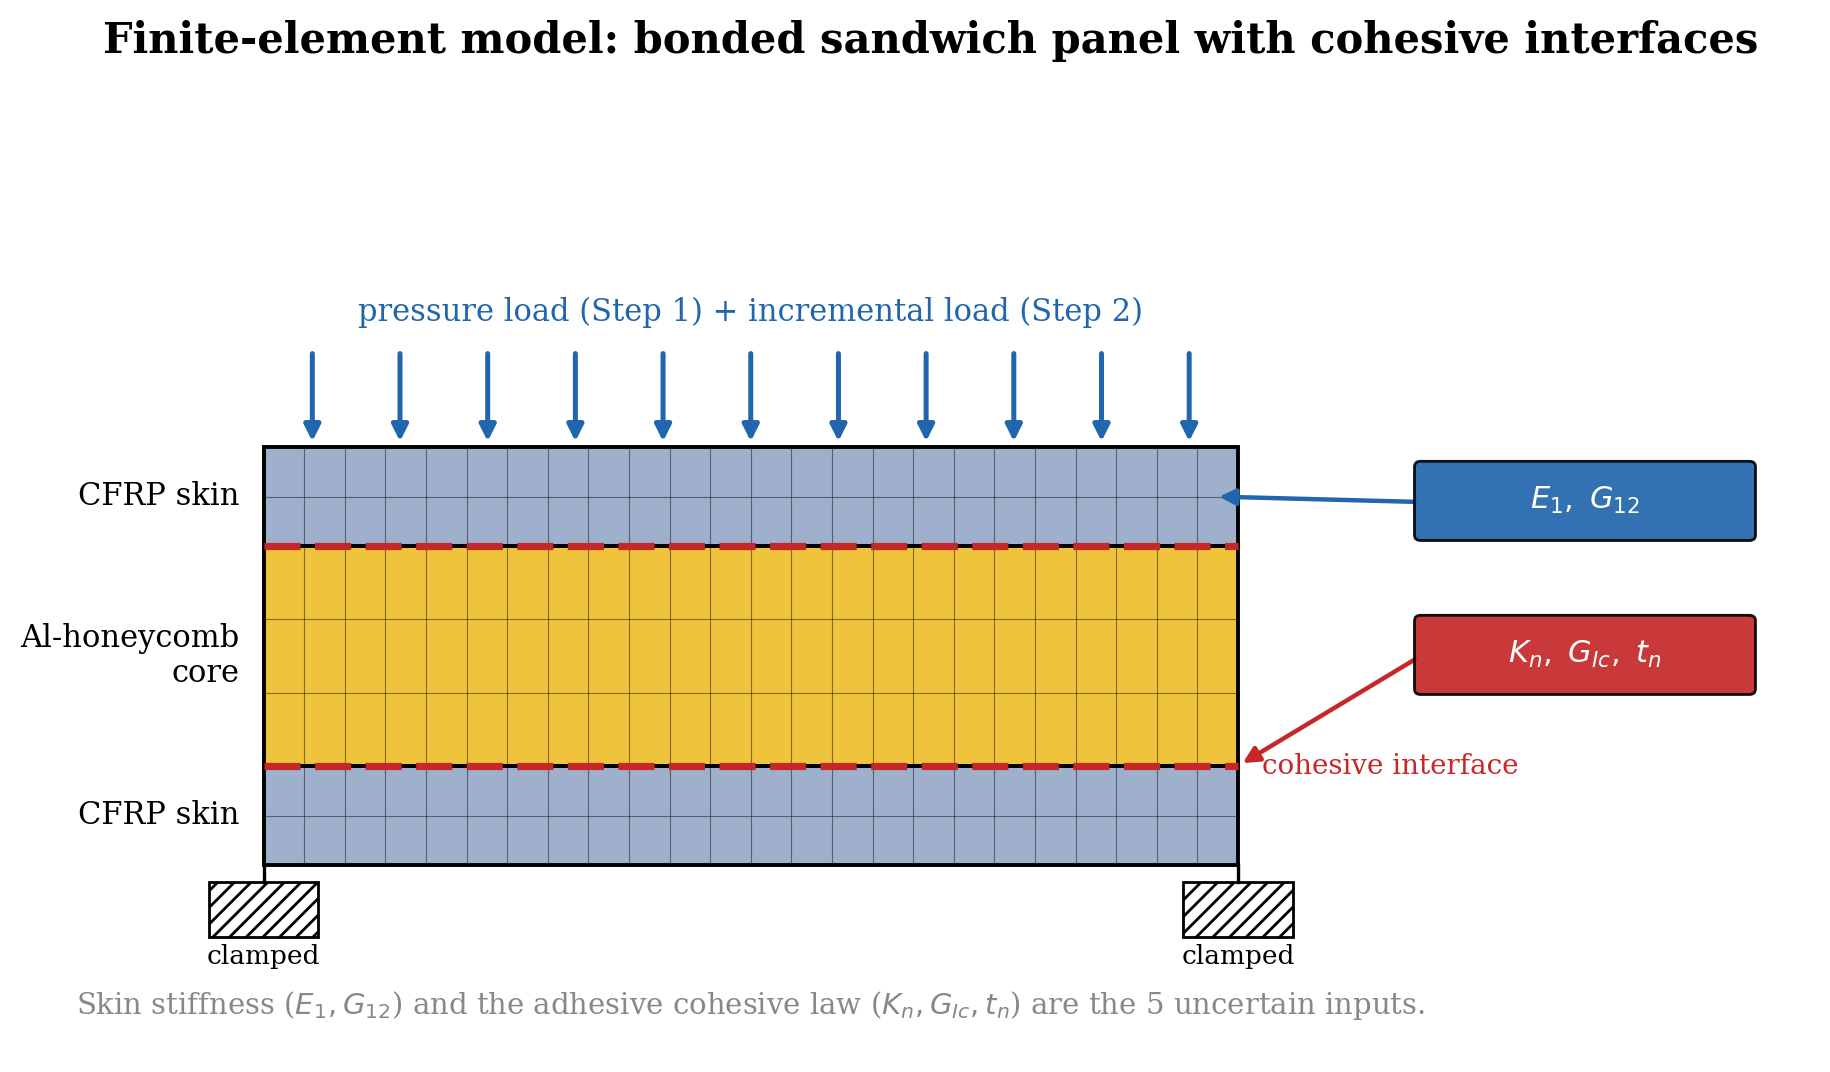
\includegraphics[height=0.80\textheight]{fem_panel_model.png}
\end{center}
\end{frame}
\note{This is the model schematic. Two carbon-fiber skins enclose an aluminum-honeycomb core, bonded by cohesive interfaces shown as the dashed red lines. The panel is clamped at its edges and loaded by pressure in the first step and an incremental load in the second. The five uncertain inputs map onto two physical locations: the skin stiffnesses E1 and G12 in the laminae, and the cohesive law Kn, GIc, and tn at the adhesive interface.}

\begin{frame}{Abaqus FE solve — von Mises stress field}
\begin{columns}[c]
\begin{column}{0.54\textwidth}
\begin{center}
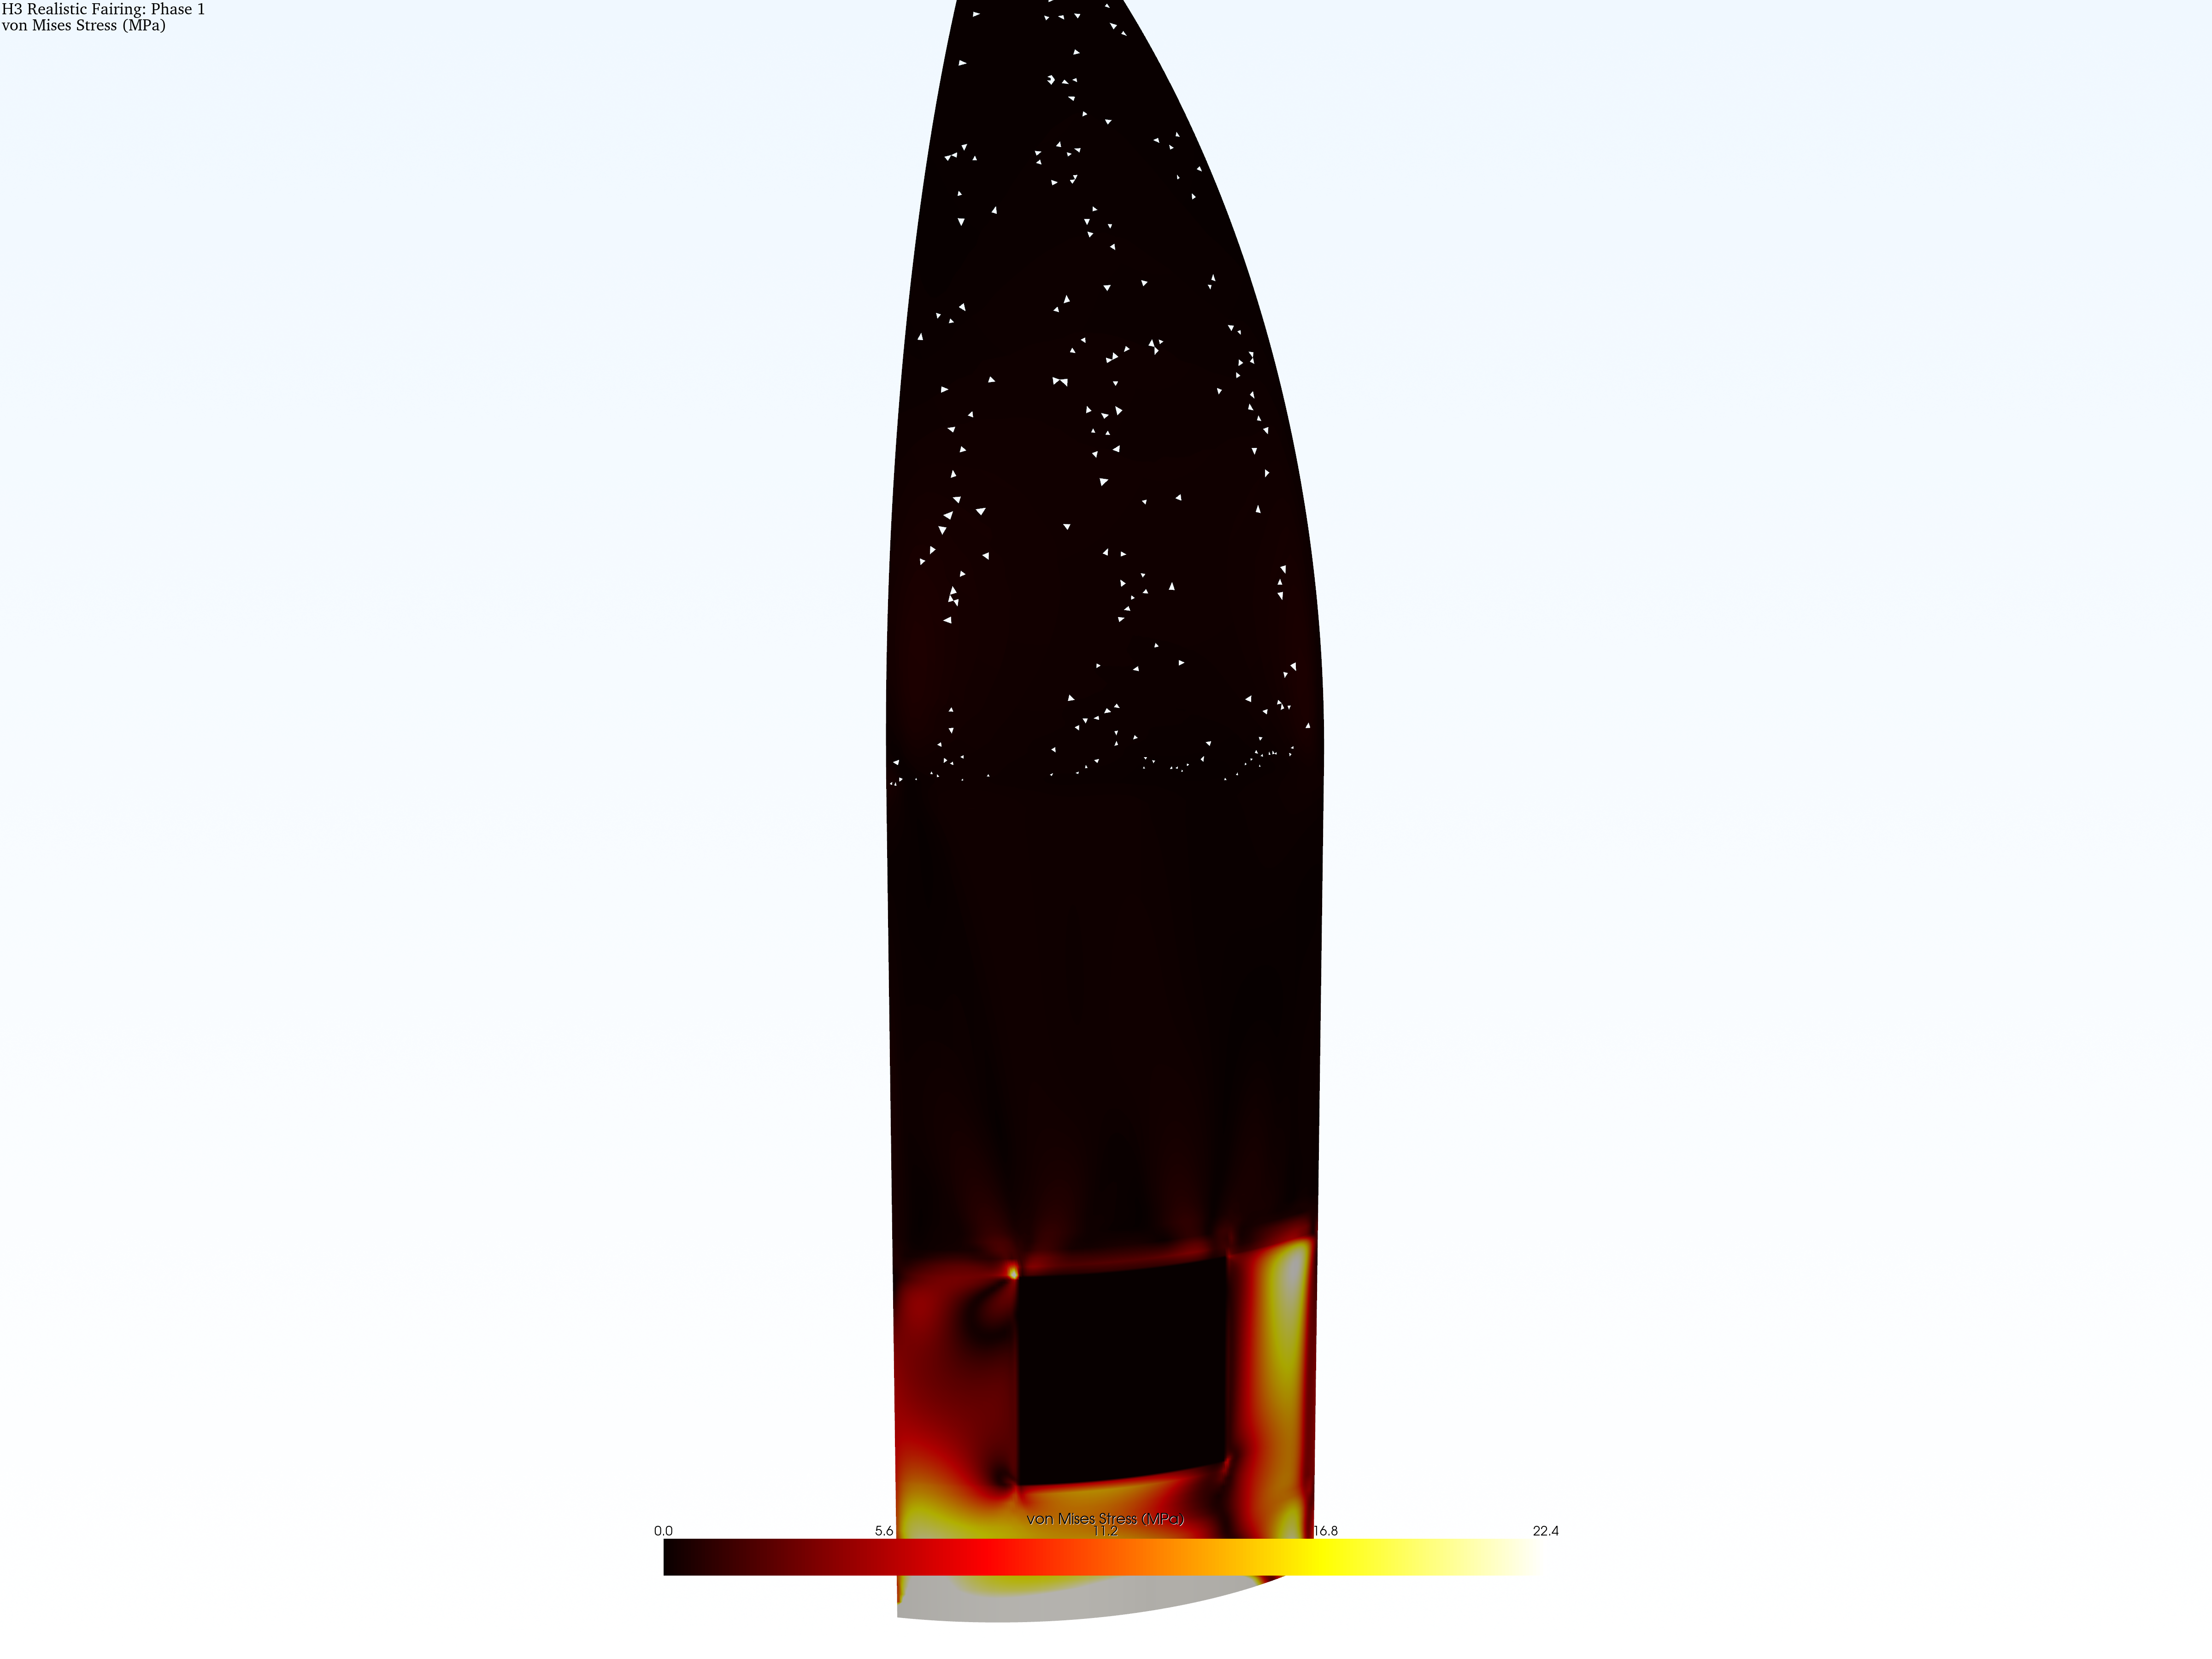
\includegraphics[height=0.82\textheight]{fairing_odb_mises.png}
\end{center}
\end{column}
\begin{column}{0.44\textwidth}
\small
\begin{itemize}
  \item Each PCE quadrature node is one \textbf{deterministic Abaqus solve}.
  \item Real \textbf{CFRP / Al-honeycomb} sandwich fairing (Abaqus ODB); von Mises peaks around the \textbf{access-door cutout}.
  \item The PCE study wraps a representative \textbf{sandwich panel} of this structure as a black box.
\end{itemize}
\end{column}
\end{columns}
\end{frame}
\note{To make concrete what one black-box evaluation looks like, this is a von Mises stress field recovered from an Abaqus output database of the full H3 fairing, with CFRP composite skins on an aluminum-honeycomb core. Each quadrature node in the polynomial-chaos construction corresponds to exactly one such deterministic solve. The stress concentrates around the access-door cutout. This global model is shown for illustration; the polynomial-chaos study itself wraps a representative sandwich panel of this structure, extracting the peak von Mises stress, the cohesive damage, and the displacement from each run.}

\begin{frame}{H3 fairing FEM — mesh and displacement}
\begin{columns}[c]
\begin{column}{0.5\textwidth}
\begin{center}
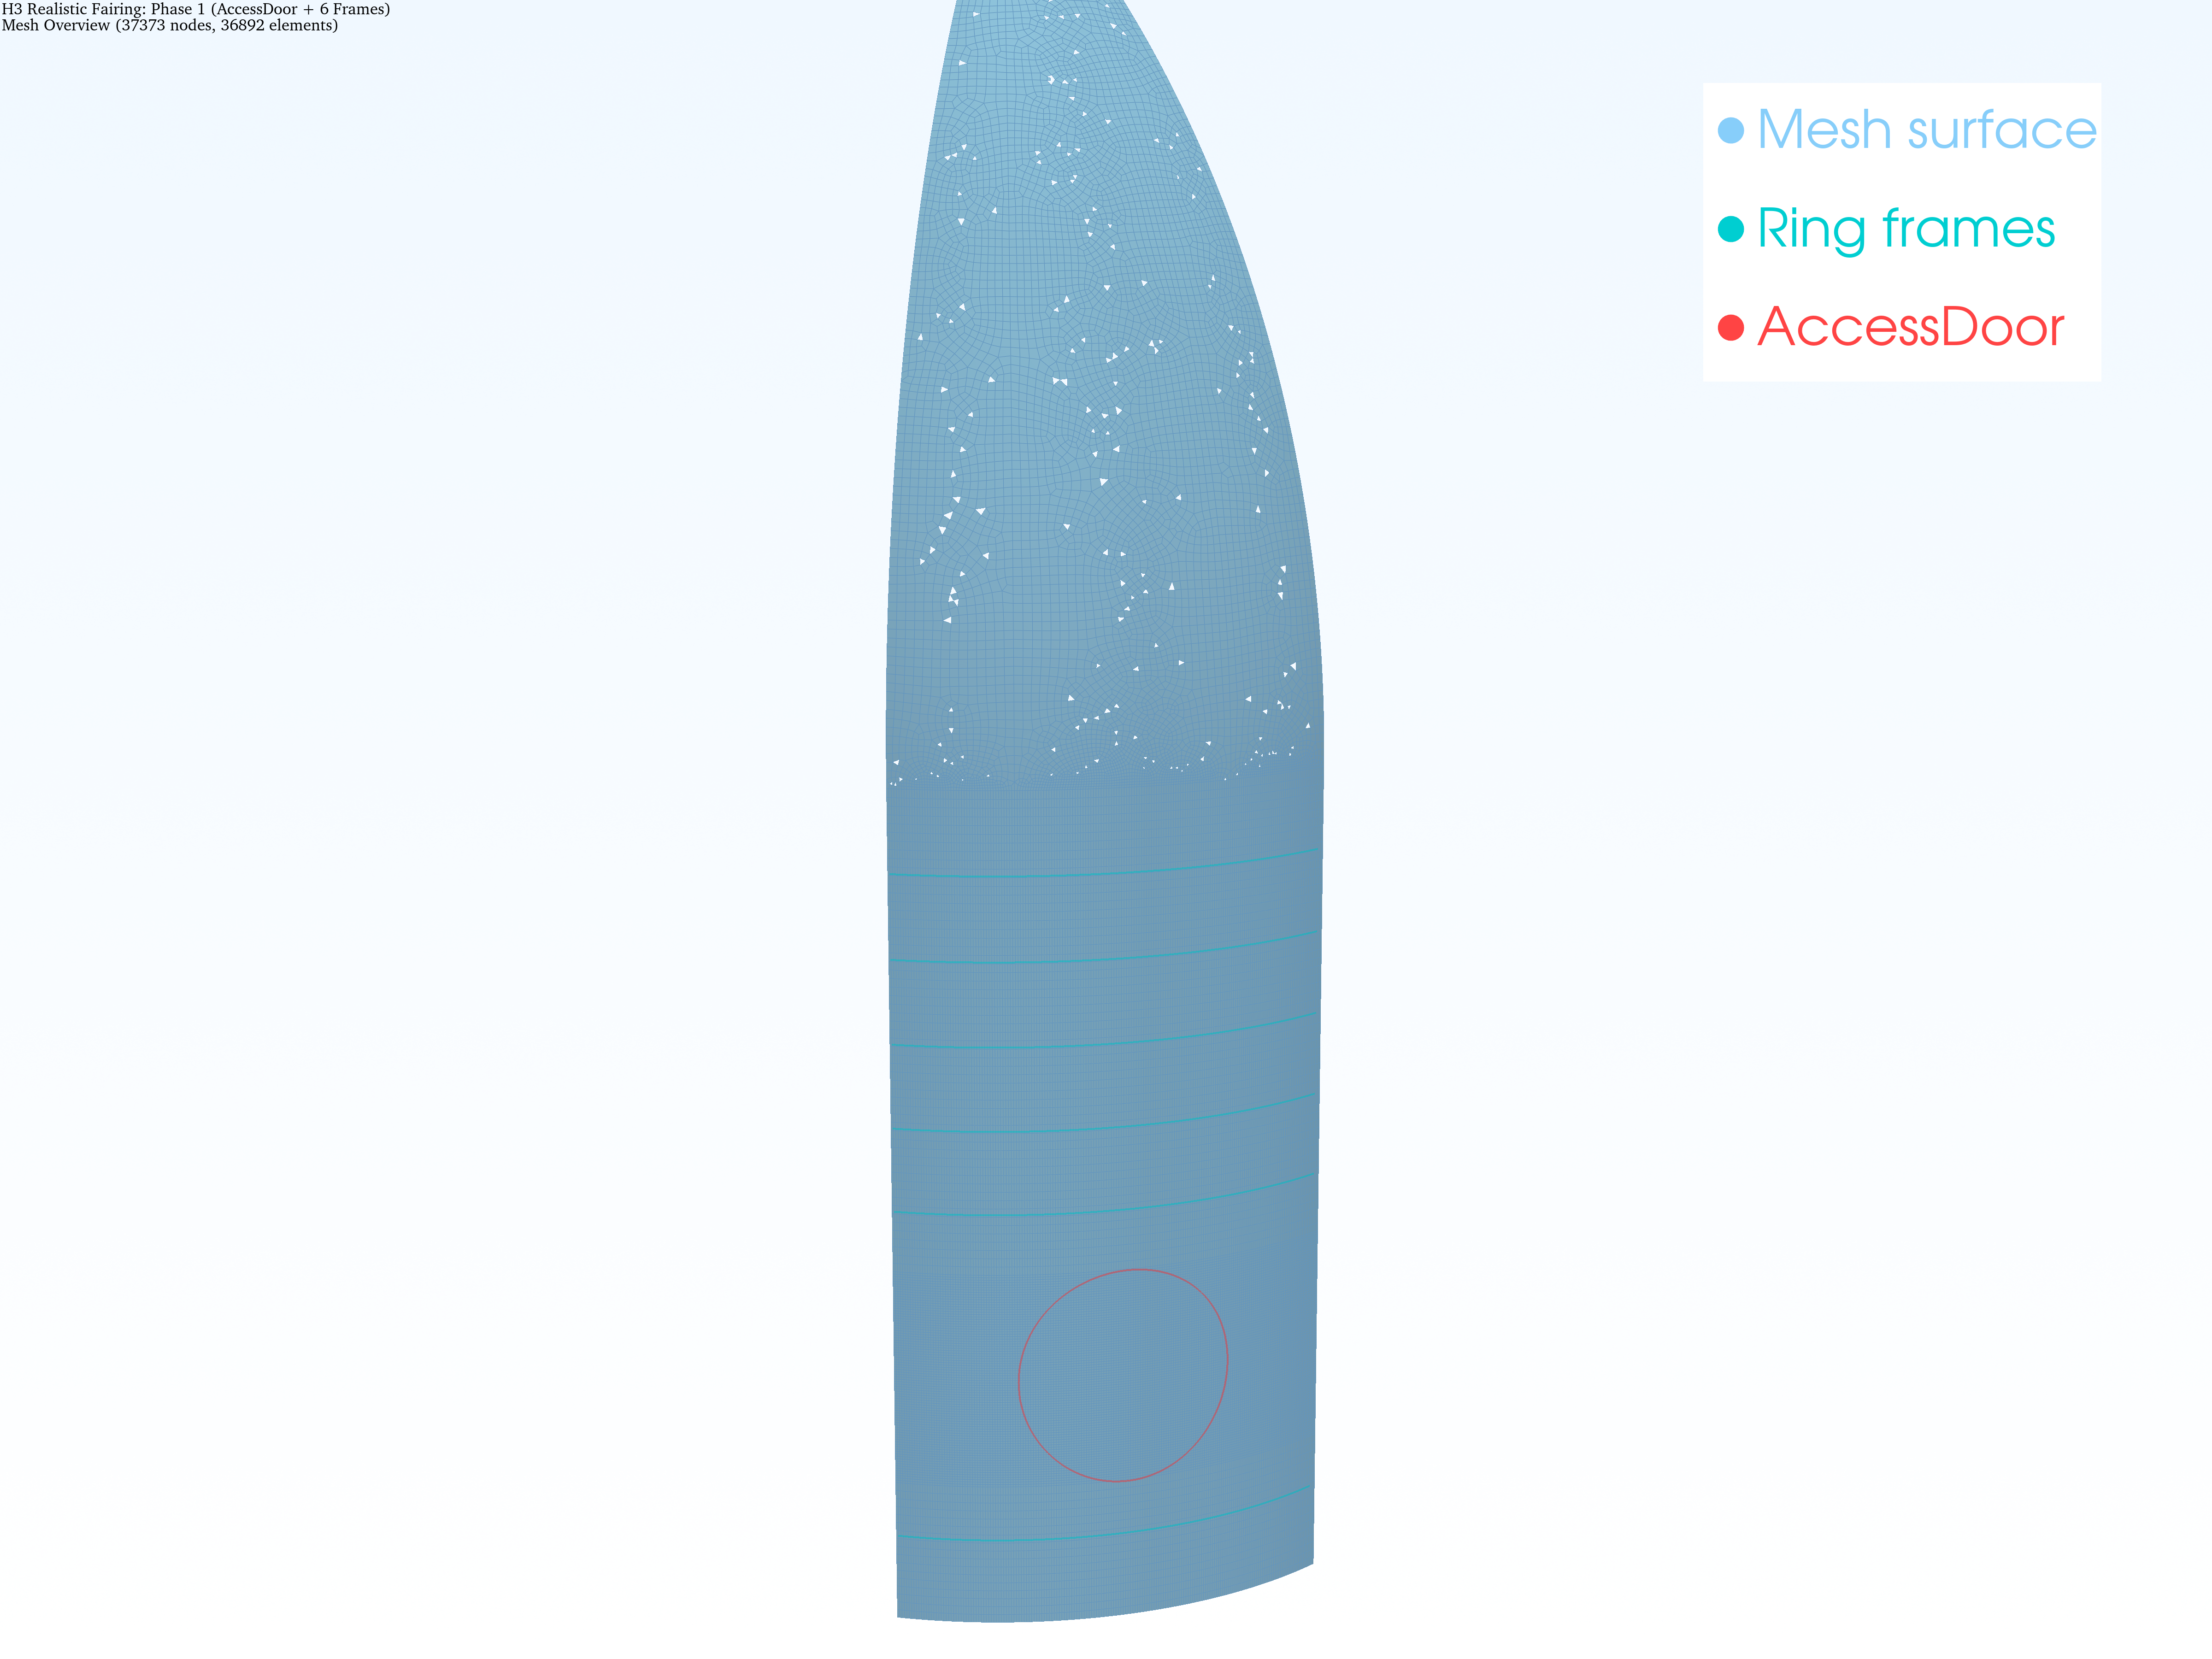
\includegraphics[height=0.80\textheight]{fairing_mesh.png}\\[-0.2em]
{\footnotesize Mesh: composite skins, ring frames, access door}
\end{center}
\end{column}
\begin{column}{0.5\textwidth}
\begin{center}
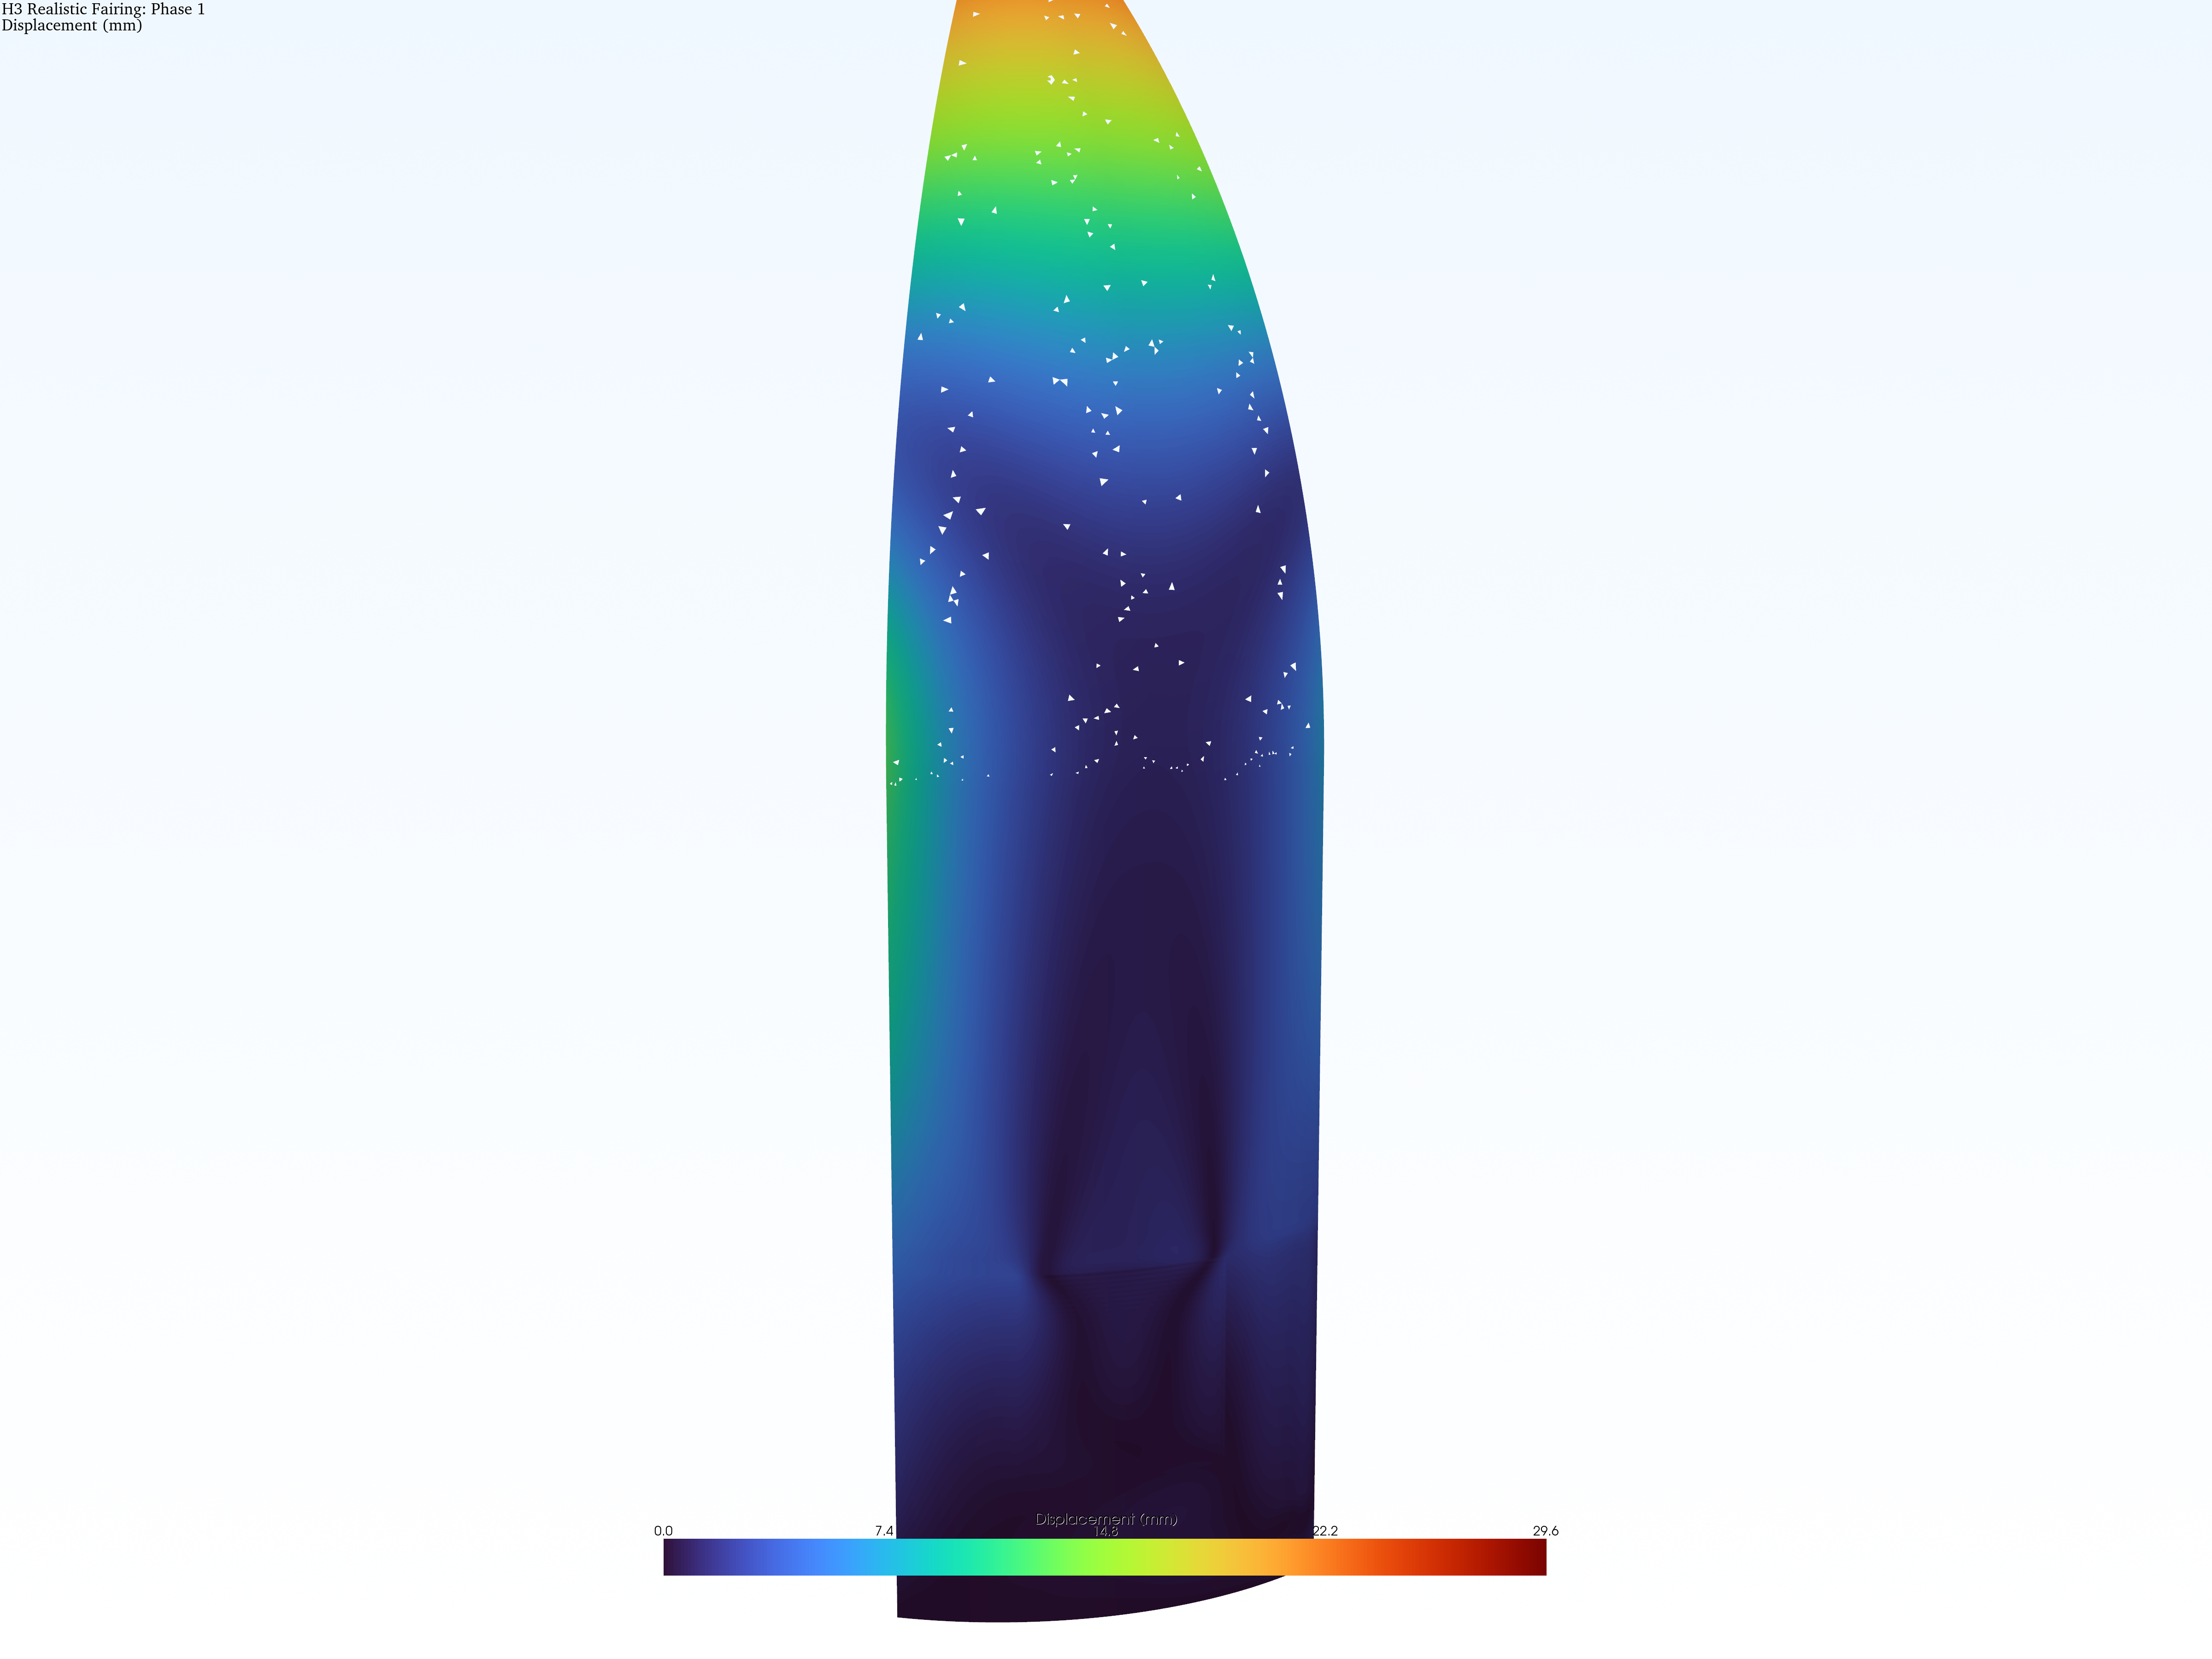
\includegraphics[height=0.80\textheight]{fairing_disp.png}\\[-0.2em]
{\footnotesize Displacement field (max at the nose tip)}
\end{center}
\end{column}
\end{columns}
\end{frame}
\note{For completeness, the left panel shows the finite-element mesh of the full fairing, with the composite skins, the ring stiffening frames, and the access-door cutout. The right panel shows the displacement field, which is largest at the nose tip. Together with the previous stress field, these illustrate the deterministic model that the polynomial-chaos surrogate wraps.}
\note{The deterministic model is an Abaqus/Standard model of a representative panel of the fairing sandwich. The CFRP skin is an orthotropic elastic lamina, the honeycomb core is linear elastic, and the adhesive interface is a cohesive-zone model with a Benzeggagh-Kenane mixed-mode damage law. The load is applied in two static steps, and the quantities of interest are extracted from the last frame through the odbAccess Python interface. There are three quantities of interest: the peak von Mises stress in the skin, with a failure limit of twelve hundred megapascals; the maximum cohesive damage variable, SDEG, with a limit of zero point five; and the maximum displacement. The whole pipeline is non-intrusive: for each quadrature node I patch the material cards in the input file, run Abaqus, extract the quantities of interest, and fit the polynomial-chaos coefficients.}

\begin{frame}{Result 1: response statistics converge at degree 2}
\begin{table}\centering\small
\begin{tabular}{lccccc}
\toprule
QoI & Mean & Std.\ Dev. & CV & $P_f$ & $\beta$ \\
\midrule
$\sigma_\text{vM}^\text{max}$ (deg 2) & 209.7 MPa & 2.375 MPa & 1.13\% & 0 & $\infty$ \\
$\sigma_\text{vM}^\text{max}$ (deg 3) & 209.7 MPa & 2.378 MPa & 1.13\% & 0 & $\infty$ \\
SDEG                                  & 0.000     & 0.000     & ---    & 0 & $\infty$ \\
$u^\text{max}$                        & 10.07 mm  & 0.178 mm  & 1.76\% & --- & --- \\
\bottomrule
\end{tabular}
\end{table}
Degree 2 (66 runs) and degree 3 (286 runs) agree to \textbf{four significant figures} $\Rightarrow$ converged. Adhesive damage is \textbf{identically zero} across all 352 simulations.
\end{frame}
\note{Now the results. The response statistics are essentially identical between degree two, built from sixty-six runs, and degree three, built from two hundred eighty-six runs --- they agree to four significant figures. That confirms the expansion has converged at degree two. The peak von Mises stress has a mean of two hundred nine point seven megapascals, with a coefficient of variation of only one point one three percent. And notably, the adhesive damage variable is identically zero across all three hundred fifty-two simulations --- the cohesive interface never initiates damage at this load.}

\begin{frame}{Result 2: $E_1$ governs over 99\% of the variance}
\begin{columns}[T]
\begin{column}{0.46\textwidth}
\begin{table}\centering\footnotesize
\begin{tabular}{lcc}
\toprule
& $S_i$ stress & $S_i$ disp. \\
\midrule
$E_1$    & \textbf{0.9921} & \textbf{0.9995} \\
$G_{12}$ & 0.0079          & 0.0005 \\
$K_n,G_{Ic},t_n$ & $\approx 0$ & $\approx 0$ \\
\bottomrule
\end{tabular}
\end{table}
{\footnotesize $S_i\approx S_T^i$: inputs act additively, no resolvable interactions.}
\end{column}
\begin{column}{0.54\textwidth}
\centering
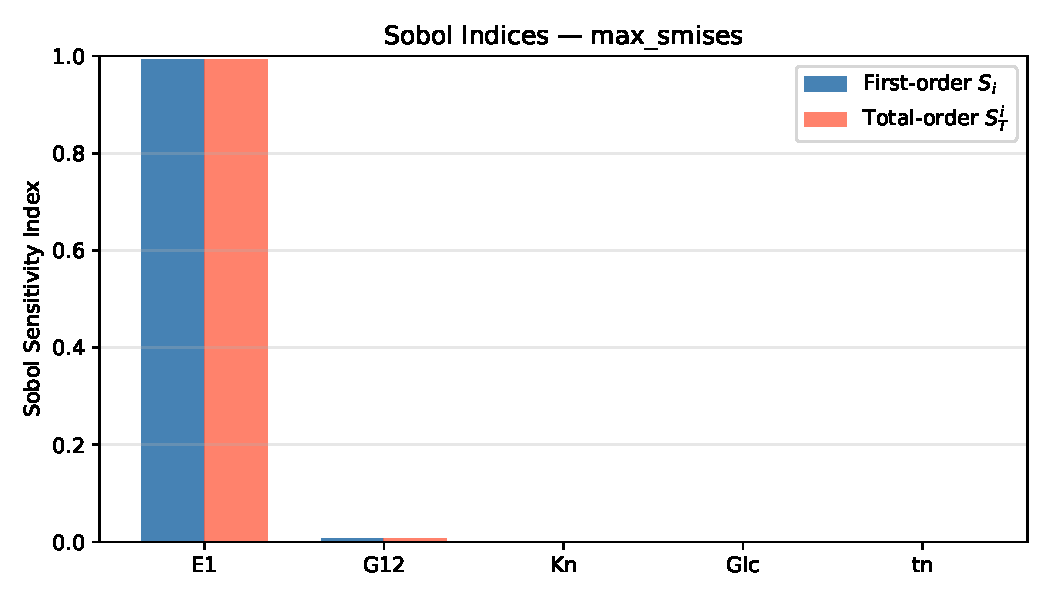
\includegraphics[width=\linewidth]{sobol_max_smises.pdf}
\end{column}
\end{columns}
\end{frame}
\note{The sensitivity analysis gives a strikingly anisotropic picture. The fiber-direction modulus E1 alone explains ninety-nine point two percent of the variance in peak stress, and ninety-nine point nine five percent of the variance in displacement. No other parameter reaches even the one-percent level. The in-plane shear modulus G12 is the only secondary contributor, and the three cohesive parameters have Sobol indices numerically indistinguishable from zero --- the direct counterpart of the damage being identically zero. The first-order and total-order indices are nearly equal, which tells us the inputs act additively with no resolvable interactions: the response is essentially linear over the sampled range.}

\begin{frame}{Why does $E_1$ dominate? A first-order argument}
\[
  \mathrm{Var}(Y) \approx \sum_{i=1}^{d}\left(\frac{\partial Y}{\partial \xi_i}\right)^2 \sigma_{\xi_i}^2
\]
\begin{itemize}
  \item Each contribution scales with \textbf{sensitivity $\times$ variance} --- not either alone.
  \item Panel carries load by \textbf{membrane action}: stress and deflection set by axial stiffness $E_1 t$ $\Rightarrow$ large $\partial Y/\partial E_1$, and $E_1$ still carries 5\% scatter.
  \item $G_{12}$ has \emph{twice} the CoV but tiny $\partial Y/\partial G_{12}$ $\Rightarrow$ suppressed.
\end{itemize}
\begin{alertblock}{}
Ranking is set by which uncertainty the structure is configured to \emph{amplify} --- not by which input is most uncertain.
\end{alertblock}
\end{frame}
\note{Why does E1 dominate? This is best understood with a first-order propagation argument, not treated as a numerical curiosity. To first order, the output variance is a sum over inputs of the squared local sensitivity times the input variance. So each parameter's contribution scales with the product of its sensitivity and its variance --- not with either one alone. The panel carries the pressure predominantly through membrane action, and both the peak stress and the deflection are set by the axial laminate stiffness, E1 times thickness. So the sensitivity to E1 is large, and E1 also carries a non-negligible five-percent scatter; the product places almost all the variance on this one parameter. The shear modulus is the instructive counter-example: it has twice the coefficient of variation, but the membrane kinematics make its sensitivity small, so that larger scatter is suppressed in the output. The ranking is governed by which uncertainty the structure is mechanically configured to amplify, not by which input is most uncertain.}

\begin{frame}{Result 3: PCE vs neural-network surrogate}
\begin{table}\centering\small
\begin{tabular}{lcccc}
\toprule
LOO RMSE & PCE deg 2 & PCE deg 3 & NN (66) & NN (286) \\
\midrule
$\sigma_\text{vM}^\text{max}$ (MPa) & $\mathbf{9.4\times10^{-4}}$ & $1.5\times10^{-3}$ & $7.2\times10^{-4}$ & $1.8\times10^{-2}$ \\
$u^\text{max}$ (mm)                 & $\mathbf{4.2\times10^{-5}}$ & $7.1\times10^{-5}$ & $2.7\times10^{-5}$ & $1.6\times10^{-3}$ \\
\bottomrule
\end{tabular}
\end{table}
\begin{itemize}\small
  \item PCE degree 2 is the most accurate; degree 3 is slightly \emph{worse} (over-parameterisation on a near-linear response).
  \item NN error \textbf{grows} an order of magnitude from 66 to 286 points --- overfitting.
  \item PCE returns Sobol indices analytically; NN would need a separate Monte Carlo study.
\end{itemize}
\end{frame}
\note{How does polynomial chaos compare with a neural network trained on the same data? The polynomial-chaos expansion at degree two attains the lowest leave-one-out error of any configuration. Tellingly, degree three performs slightly worse --- fitting fifty-six coefficients to two hundred eighty-six points introduces estimation variance in redundant high-order terms, the classic symptom of mild over-parameterisation on an almost-linear response. The neural network shows the same pathology far more sharply: its out-of-sample error grows by an order of magnitude when the training set is enlarged from sixty-six to two hundred eighty-six points, because a fixed network with several thousand weights overfits when the underlying map is this smooth. This is not a generic claim that polynomial chaos beats neural networks; it is a statement about the match between method and problem. Polynomial chaos encodes a strong prior --- that the response is a low-order polynomial --- and when that prior is correct it extracts accurate statistics from very few samples and returns the sensitivity indices for free.}

\begin{frame}{Reliability: a wide margin, and an unidentifiable interface}
\begin{columns}[T]
\begin{column}{0.5\textwidth}
\centering
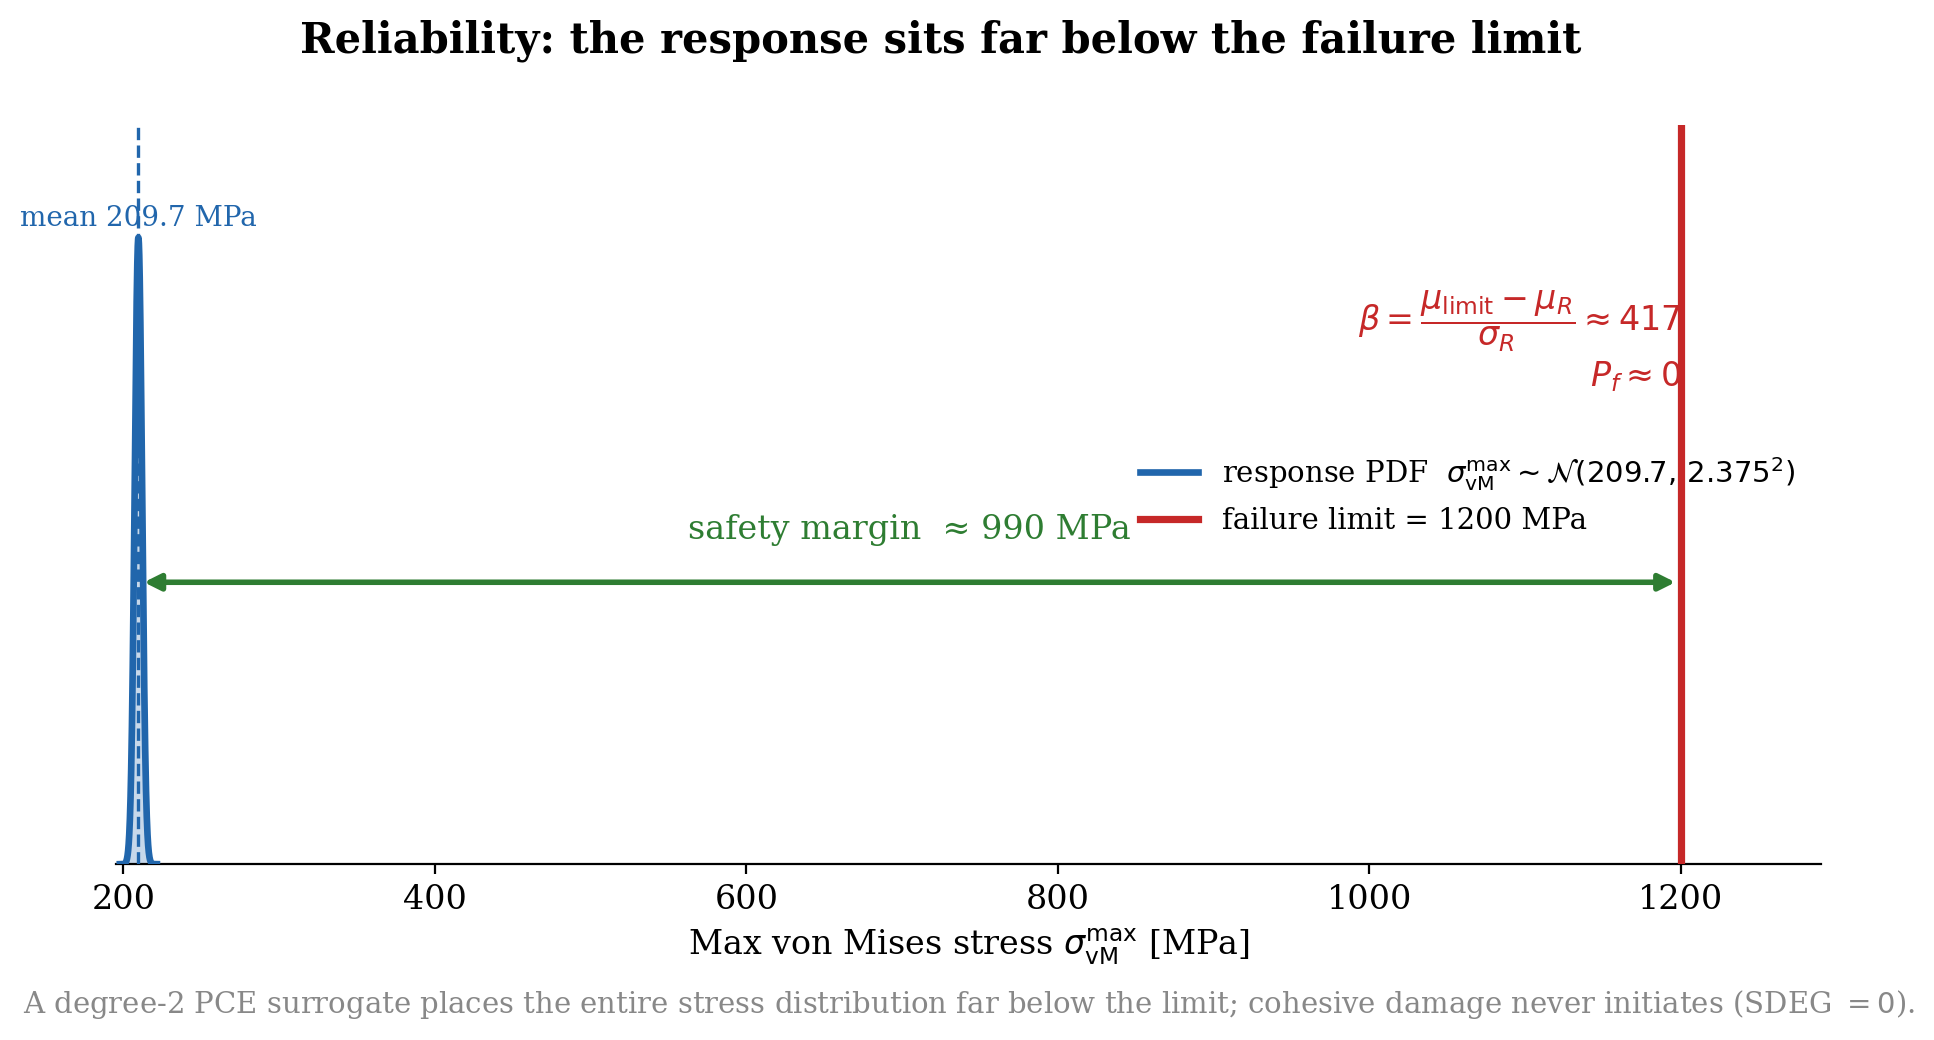
\includegraphics[width=\linewidth]{reliability_margin.png}
\end{column}
\begin{column}{0.5\textwidth}
\[
  P_f = P(\sigma_\text{vM}^\text{max}>1200) = 0,\quad \beta=\infty
\]
\begin{itemize}\small
  \item Mean stress is $(1200-209.7)/2.38 \approx \mathbf{416\sigma}$ below failure.
  \item Read $P_f=0$ as ``\textbf{below the resolution} of the analysis'' (MC of $10^6$; inputs truncated at $\pm50\%$).
  \item SDEG $\equiv 0$ $\Rightarrow$ cohesive parameters are \textbf{structurally unidentifiable} at this load.
\end{itemize}
\end{column}
\end{columns}
\end{frame}
\note{Now reliability. Monte Carlo sampling of a million realisations on the surrogate gives a failure probability of zero and an infinite reliability index. The mean stress sits about four hundred sixteen standard deviations below the failure threshold. But I want to state this carefully: a failure probability of exactly zero should be read as below the resolution of the analysis, not as a literal guarantee. The Monte Carlo can only resolve probabilities down to about ten to the minus six, and more fundamentally the surrogate is only valid over inputs truncated at plus or minus fifty percent of nominal; genuine tail risk lies outside that range, where the polynomial cannot be trusted to extrapolate. There is also a methodological consequence of the damage being identically zero: the three cohesive parameters are structurally unidentifiable in this study. Because they never move any output, no amount of sampling could give them a non-zero Sobol index, and the nominally five-dimensional problem collapses, at this load, to an effectively one-dimensional problem in E1.}

\begin{frame}[t]{Extension T9: scalar $E_1$ is conservative --- KL random field}
\begin{columns}[T]
\begin{column}{0.54\textwidth}
\vspace{0.3em}
Represent $E_1(x,y)$ as a Gaussian random field with anisotropic exponential covariance:
\[
  C = \sigma_{E_1}^2\,e^{-|dx|/l_{cx}-|dy|/l_{cy}}
\]
Discretise via \textbf{KL expansion}; compute std.\ of the spatial mean $\overline{E_1}$.
\vspace{0.5em}

\textbf{Key result:} $\sigma(\overline{E_1})\approx 5{,}100$~MPa $<$ scalar $\sigma_{E_1}=7{,}300$~MPa.
\begin{alertblock}{}
Spatial averaging attenuates variability $\Rightarrow$ scalar UQ is \textbf{conservative}.
\end{alertblock}
\end{column}
\begin{column}{0.46\textwidth}
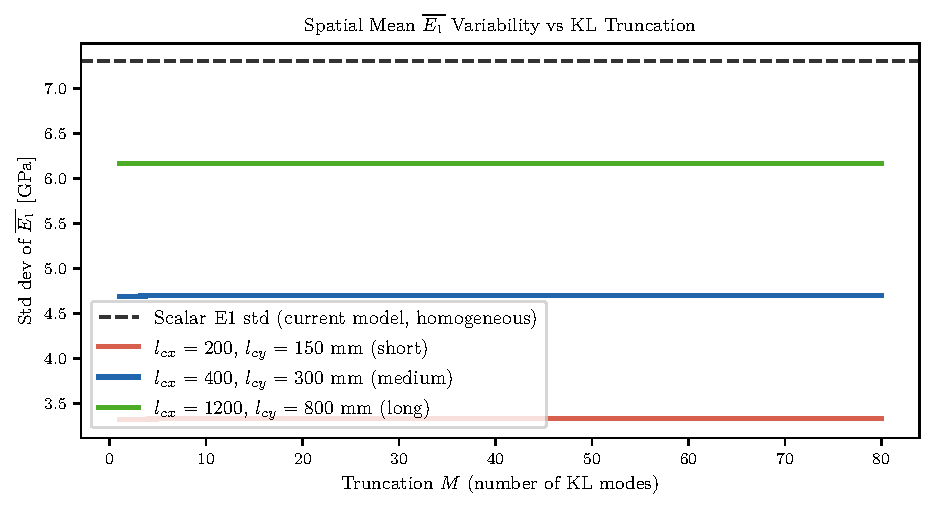
\includegraphics[width=\linewidth]{kl_effective_variance.pdf}
\end{column}
\end{columns}
\end{frame}
\note{Extension Topic 9: I replace the scalar E1 assumption with a spatially varying random field, discretised via Karhunen-Loeve expansion using an anisotropic exponential covariance kernel. The key question is whether the scalar model over- or underestimates the structural variability. The answer is that it overestimates: the effective standard deviation of the spatially averaged E1, which drives the panel response, is about five thousand one hundred megapascals for a realistic correlation length, compared to seven thousand three hundred for the scalar. Spatial averaging attenuates variability. So the scalar analysis used in the core study is conservative, and the true reliability is even better than computed. The figure shows the effective standard deviation as a function of the number of retained KL modes, for three correlation length cases; all converge well below the scalar baseline.}

\begin{frame}[t]{Extension T13: PCE achieves exact recovery --- surrogate comparison}
\begin{columns}[T]
\begin{column}{0.55\textwidth}
\vspace{0.3em}
Compare \textbf{PCE} (deg.~1/2), \textbf{GP} (RBF kernel), \textbf{NN} (MLP) as a function of training size $N=10$--$286$. Median RMSE over 5 seeds.
\vspace{0.4em}

\begin{table}\centering\footnotesize
\begin{tabular}{lc}
\toprule
Surrogate & RMSE at $N{=}66$ \\
\midrule
PCE deg.\ 2 & $3\times10^{-13}$ MPa \\
GP          & $7\times10^{-4}$\ MPa \\
NN          & $3.6\times10^{-1}$\ MPa \\
\bottomrule
\end{tabular}
\end{table}
PCE deg.~2 achieves \textbf{machine precision}: exact polynomial recovery.
\end{column}
\begin{column}{0.45\textwidth}
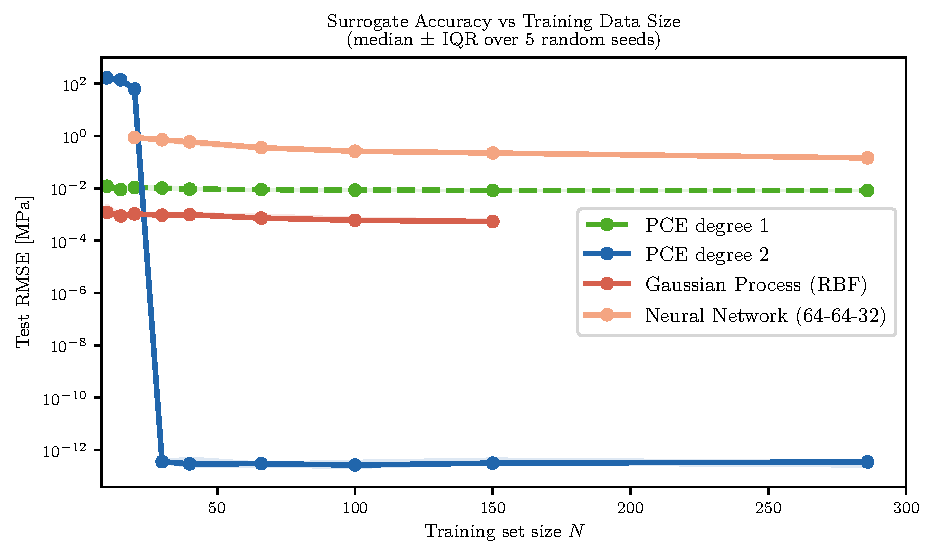
\includegraphics[width=\linewidth]{t13_rmse_convergence.pdf}
\end{column}
\end{columns}
\end{frame}
\note{Extension Topic 13: I systematically compare polynomial chaos, Gaussian process, and neural network surrogates over training set sizes from ten to two hundred eighty-six points. At N=66, PCE degree two achieves machine-precision RMSE --- ten to the minus thirteen megapascals --- because the underlying response is itself a degree-two polynomial in the Gaussian inputs, and the PCE recovers the exact representation. The GP reaches seven times ten to the minus four megapascals, which is very good but not exact, because the kernel prior doesn't match the polynomial truth. The neural network is five hundred times worse than the GP, exhibiting the classic overfitting signature on a smooth low-variance response. The figure shows all four curves; the GP epistemic uncertainty band (not shown here) is less than five percent of the aleatory variance at N=66, confirming that surrogate error is negligible.}

\begin{frame}[t]{Extension T6: $E_1$ dominance $\Rightarrow$ tractable Bayesian identification}
\begin{columns}[T]
\begin{column}{0.55\textwidth}
\vspace{0.3em}
PCE linear term: $\hat\sigma_\text{vM} = 209.7 + 2.365\,\xi_{E_1}$~MPa.

Conjugate Gaussian update given $k$ stress measurements:
\[
  \sigma_\text{post}(E_1) = \frac{\sigma_{E_1}}{\sqrt{1+k\,c_1^2/\sigma_\text{meas}^2}}
\]

\vspace{0.3em}
\textbf{Key result:} $k=5$ measurements reduce $\sigma_{E_1}$ from 7{,}300 to 5{,}300~MPa (-27\%); $k=20$ gives -74\%.
\begin{alertblock}{}
PCE doubles as the engine of a \textbf{real-time QC feedback loop}.
\end{alertblock}
\end{column}
\begin{column}{0.45\textwidth}
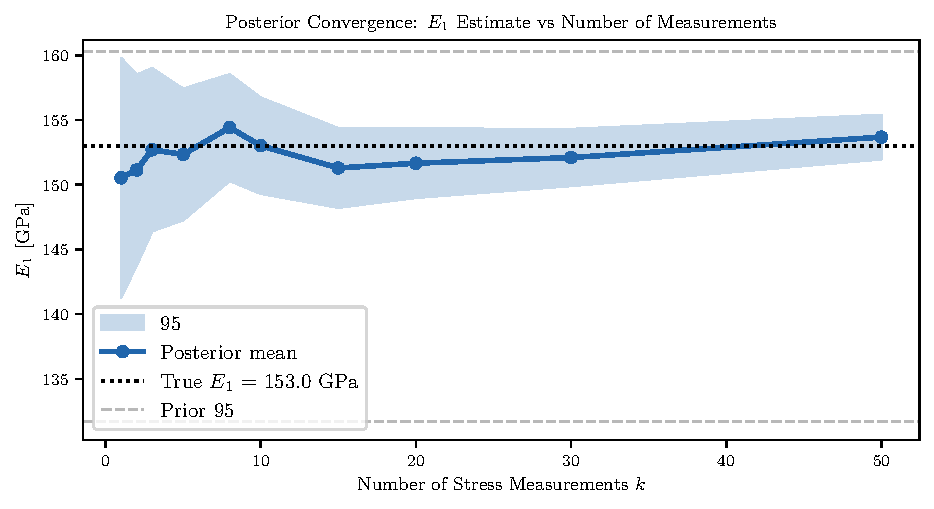
\includegraphics[width=\linewidth]{bayes_convergence_k.pdf}
\end{column}
\end{columns}
\end{frame}
\note{Extension Topic 6: the Sobol result says E1 explains ninety-nine percent of the output variance. That means E1 is also the most identifiable parameter: if you can measure the stress on a panel, you can infer E1. I set this up as a conjugate Gaussian inverse problem, using the PCE linear approximation as the likelihood. No new Abaqus runs are needed. With just one observation, the posterior standard deviation drops from seven thousand three hundred to about four thousand seven hundred megapascals. Five measurements give a twenty-seven percent reduction; twenty measurements give seventy-four percent. The figure shows the posterior mean and ninety-five percent credible interval converging to the true E1 as the number of measurements grows. The implication is that the PCE surrogate is not just a forward propagation tool --- it doubles as the engine of a real-time statistical process control loop: as batches are tested and stress measurements accumulate, the E1 distribution is progressively refined.}

\begin{frame}{Conclusions \& limitations}
\begin{itemize}
  \item PCE deg.~2 (66 runs) converged; \textbf{$E_1$ controls $>99\%$} of variability; panel reliable ($\beta=\infty$).
  \item \textbf{T9}: spatial averaging in KL field attenuates variability $\Rightarrow$ scalar UQ is conservative.
  \item \textbf{T13}: PCE achieves exact recovery ($3\!\times\!10^{-13}$~MPa RMSE); NN 500$\times$ worse at $N{=}66$.
  \item \textbf{T6}: PCE doubles as a Bayesian QC loop --- 5 measurements $\Rightarrow$ 27\% posterior reduction.
\end{itemize}
\vspace{0.2em}
\begin{alertblock}{Honest limitations}
$P_f=0$ is resolution-limited; inputs assumed independent; single panel, not full fairing; cohesive parameters unidentifiable at this load. \textbf{Next:} activate cohesive zone; correlated KL field; full-fairing geometry.
\end{alertblock}
\end{frame}
\note{To conclude. A degree-two expansion from only sixty-six simulations already captures the full response statistics, and I argue this is the correct model order for this smooth, near-linear response, not merely an economy measure. The single actionable message is that the fiber-direction modulus controls more than ninety-nine percent of the structural variability, so tightening the quality control of E1 --- through fiber-volume-fraction and cure consistency --- is by far the most effective lever for reducing variability. Under the design load the panel is reliable by a wide margin and the cohesive interface stays elastic. I will end on the honest limitations: the zero failure probability is resolution-limited; the inputs are assumed independent whereas CFRP elastic constants are physically correlated; only a single panel is modeled, not the full fairing; and only aleatory material uncertainty is propagated, not the model's own discretisation error. The natural continuation is to repeat the analysis at a load level that activates the cohesive zone, under a correlated input model and a full-fairing geometry, so that the reliability of the bonded interface itself can be assessed. Thank you very much for your attention.}

\end{document}
